% cosa fa il server mole (fa solo scrittura)
% descrizione di come viene gestita una richiesta
% mole-contact: per linguaggio
% schema delle comunicazioni e dei messaggi interni (con le code rabbit)

% autenticazione sull'api (?)
% come funziona la storia id/key per autenticarsi sulle api

% parlare di come vengono storati i dati in mongo

% parlare di come è stato usato rabbit
% configurazione rabbit utilizzata per scalare (broadcast+loadbalancing)

\begin{figure}[h]
\centering
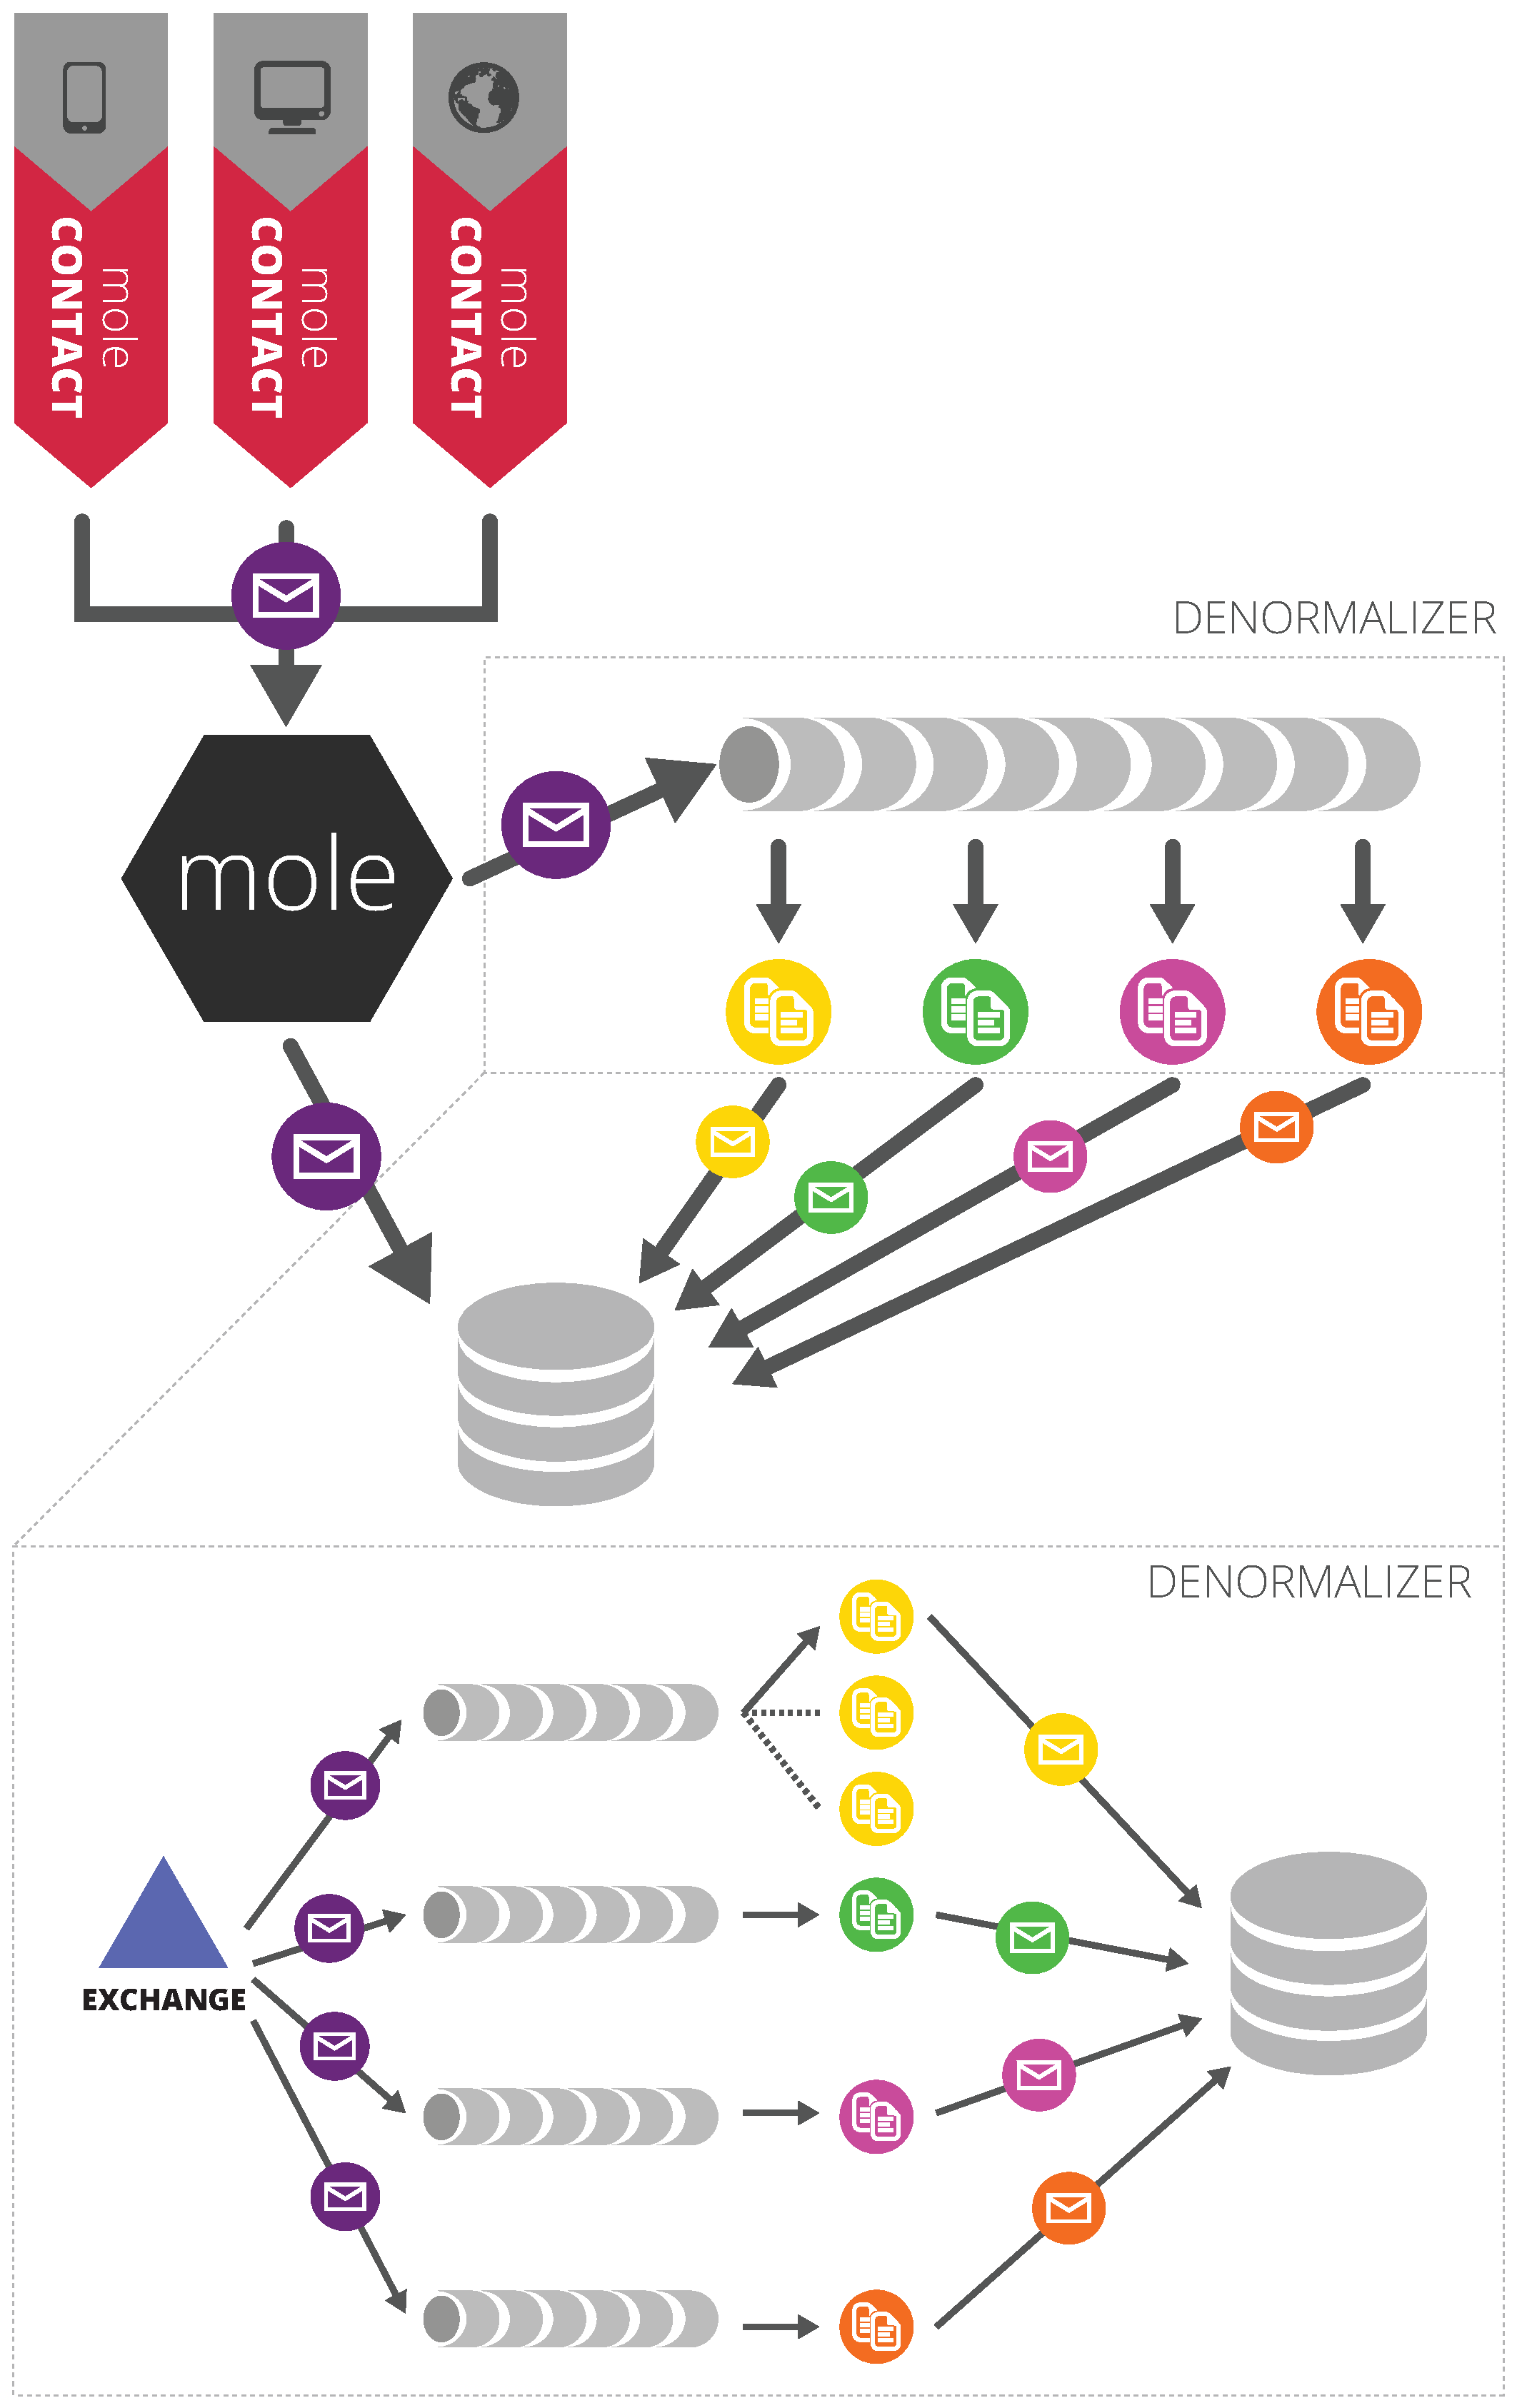
\includegraphics[width=1.0\linewidth]{./img/mole}
\caption[Architettura di mole]{Architettura di mole}
\label{fig:mole}
\end{figure}

 garantisce l'estensibilità del sistema, in quanto permette di gestire funzionalità di elaborazione dati aggiuntive, utilizzabili a fr



posso denormalizzare dati esistenti, fornisco funzionalità agli utenti in modo graduale

i denormalizzatori possono essere aggiunti nel tempo